\documentclass[dvipdfmx]{jsarticle}
\usepackage[dvipdfmx]{graphicx}
\usepackage{amsmath, amssymb}
\usepackage{mathtools}
\usepackage{here}
\begin{document}
\title{週間進捗報告}
\author{権藤陸}
\maketitle
\section{進捗}
\begin{itemize}
    \item CL法を用いたrange-angle mapのサンプルコードの理解 → range fftとdoppler fftを実装途中
    \item "Sparsity Based Non-Contact Vital Signs Monitoring of Multiple People Via FMCW Radar"の概要把握 
\end{itemize}

\section{レンジアングルマップ}
石川さんのコードを実行し,CFARの効果について確認した.レーダは中心周波数が79 GHz, 3 × 4のアンテナで計測時間は60 s, 帯域幅は3.4391 GHz, サンプリングレートは160 Hzである.

\begin{table}
    \caption{FMCWレーダ実験諸元}
    \centering
    \begin{tabular}{cc}
        \hline
        送信アンテナ数 & 3 \\
        受信アンテナ数 & 4 \\
        中心周波数 & 79 GHz \\
        帯域幅 & 3.4391 GHz \\
        サンプリングレート & 153.8 Hz\\
        \hline
    \end{tabular}
\end{table}

\begin{table}
    \caption{CFAR実験諸元}
    \centering
    \begin{tabular}{cc}
        \hline
        ガードセル長(距離)& 3 \\
        ガードセル長(角度)& 7 \\
        トレーニングセル長(距離)& 5\\
        トレーニングセル長(角度)& 7 \\
        \hline
    \end{tabular}
\end{table}


\begin{figure}[htbp]
\begin{center}
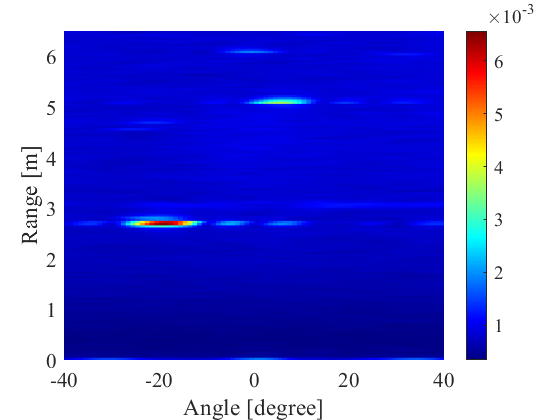
\includegraphics[width=0.8\linewidth]{./img/range_doppler_sample.png}
\end{center}
\caption{レンジアングルマップ(CFARなし)}
\end{figure}

% \begin{figure}[htbp]
% \begin{center}
% 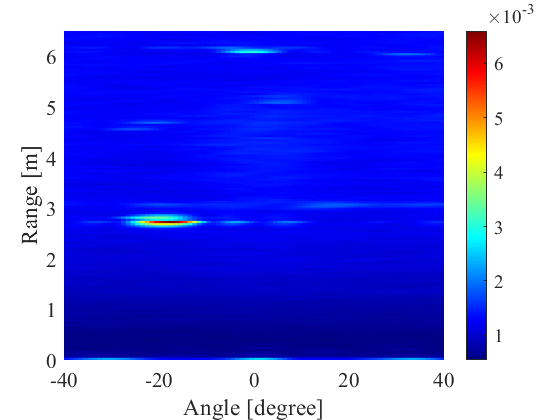
\includegraphics[width=0.8\linewidth]{./img/cfar2.png}
% \end{center}
% \caption{レンジアングルマップ(CFARあり)}
% \end{figure}

\begin{figure}[H]
\begin{center}
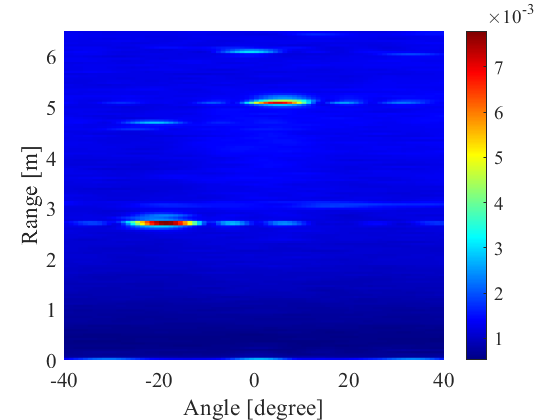
\includegraphics[width=0.8\linewidth]{./img/cfar1.png}
\end{center}
\caption{レンジアングルマップ(CFARあり)}
\end{figure}

\section{論文の概要[1]}
従来のFMCWレーダを用いた非接触バイタルサインモニタリング(NCVSM)技術は、単純化されたモデルに基づいており、複数の物体を含むノイズ環境に対する対処が困難であることが指摘されている.

複数の人物やクラッタが存在するノイズ環境におけるFMCWレーダ信号の拡張モデルとNCVSM(Non-Contact Vital Signs Monitoring)という入力データに含まれるバイタルサインの空間的スパース性を利用した新たなアプローチを提案する.
特徴として,単一チャネルで,入力出力ともに単一であること(SISO:Single-Input Single-Output)が挙げられる.
本研究は,取得したレーダ信号を入力し,最終的に人間の呼吸数と心拍数の推定を目的とする.

\section{論文の提案法[1]}
\begin{figure}[H]
\begin{center}
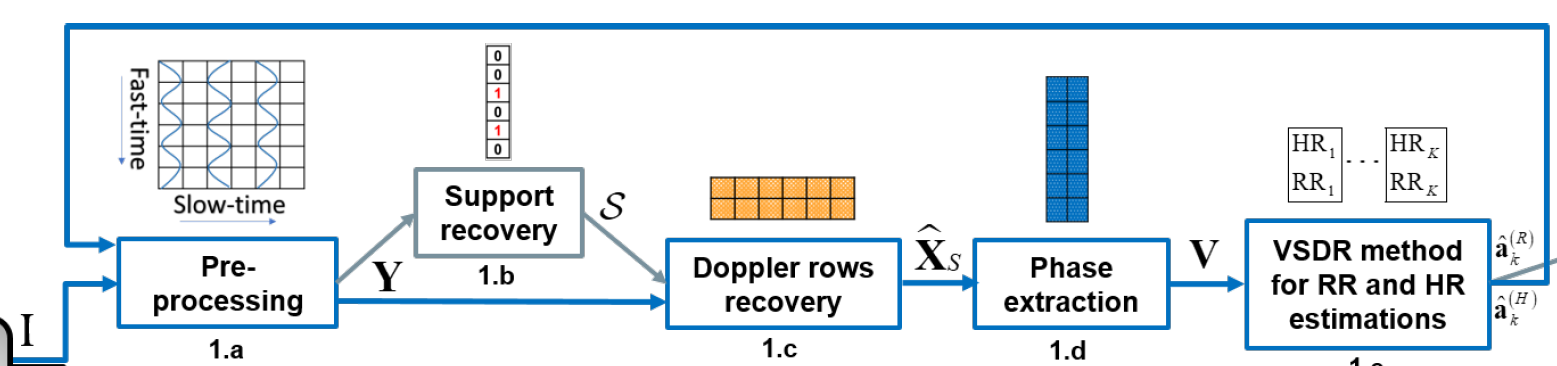
\includegraphics[width=0.8\linewidth]{./img/NCVSM_diagram.png}
\end{center}
\caption{NCVSMの流れ}
\end{figure}
\begin{itemize}
    \item 前処理(図1のPre-processing)

ビート信号を1フレームごとに平均化することで,ノイズを低減.そして,人間の典型的な脈拍と呼吸の周波数の事前知識を用いて,静的ないし振動するクラッタからバイタルサインを分離する目的で,slow-time方向にスペクトルフィルタリングを行う.

    \item FISTAアルゴリズムを用いたJoint Sparse Recovery(図1のSを求める)

ノイズが含まれた信号を復元するため,以下の式で表される最適化問題を解くために原情報推定のための再構成アルゴリズムの一つである,FISTAアルゴリズム[2][3]が用いられる.
    \item Sを用いてレーダからの距離を計算

Sは一つ前のステップで求めた,レーダより各人間の半径方向の距離を検出可能な集合であり,座標の情報(行座標)を含む?
    \item Least-Squares problem[4]から$\mathrm{F_s}と入力\mathrm{Y}を用いて図1の\mathrm{\hat{X_s}}$を求める
\begin{figure}[H]
\begin{center}
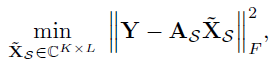
\includegraphics[width=0.35\linewidth]{./img/equation3.png}
\end{center}
\end{figure}
\begin{figure}[htbp]
\begin{center}
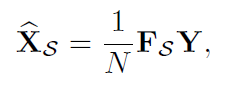
\includegraphics[width=0.2\linewidth]{./img/equation4.png}
\end{center}
\end{figure}

このステップでは,各被験者のドップラー情報を求める.被験者は呼吸や話をしているが,静止している前提である.$\mathrm{F_s}$は,fast-timeの周波数に対応する離散フーリエ変換行列の一部である
    \item 以下の式からXsを用いて図1のVを求める
\begin{figure}[htbp]
\begin{center}
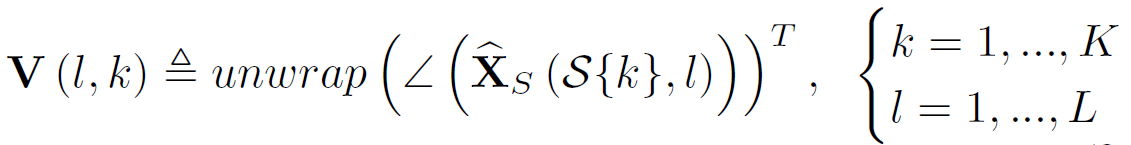
\includegraphics[width=0.6\linewidth]{./img/equation2.png}

\end{center}
\end{figure}
関連研究の"unwrap"[5]とarctanを用いて,$\hat{\mathrm{X_s}}$から位相情報を抽出し,胸部の振動に関する行列Vを求める.
    \item 呼吸数と心拍数をVSDR(Vital Signs Dictionary Recovery)と呼ばれる手法で推定する.

Dictionary-based approachについて調べる.
\end{itemize}

\section{計画}
\begin{itemize}
    \item dopper-range mapとcfarを実装
    \item 論文の疑問点解消
    \item 関連研究のサーベイ
\end{itemize}
\begin{thebibliography}{}
\item Yonathan Eder, \textit{Graduate Student Member, IEEE, }and Yonina C. Eldar, \textit{Fellow, IEEE}, "Sparsity Based Non-Contact Vital Signs Monitoring of Multiple People Via FMCW Radar", arXiv:, 2205.05152v1 [eess.SP], 10 May 2022
\item A. Beck, and M. Teboulle, “A fast iterative shrinkage-thresholding algorithm
for linear inverse problems,” SIAM journal on imaging sciences,
vol. 2, no. 1, pp. 183–202, 2009.
\item D. P. Palomar, and Y. C. Eldar, Convex optimization in signal processing and communications, Cambridge Univ. Press, 2010.
\item D. Ruppert, and M. P. Wand, “Multivariate locally weighted least squares
regression,” The annals of statistics, pp. 1346–1370, 1994.
\item M. Alizadeh, G. Shaker, J. De Almeida, P. Morita, and S. Safavi-Naeini, “Remote monitoring of human vital signs using mm-wave FMCW radar,” IEEE Access, vol. 7, pp. 54958–54968, 2019.
\end{thebibliography}
\end{document}